\section{Introduction}

The LISA space-borne Gravitational Wave Observatory\,\cite{Bender00}, when operational,
will provide a unique view of the universe at spectral frequencies unobservable
with ground based detectors. As well as directly observing the gravitational radiation from a
number of known sources, LISA will also provide the opportunity to observe unexpected
signals and sources.

In order to detect the known sources with a high signal-to-noise ratio, the strain
sensitivity of LISA has to be of the order of $10^{-21}/\sqrt{\rm Hz}$ at milliHertz
frequencies. Many of the technologies required to build an instrument that
can achieve such a strain sensitivity are currently being constructed and will
be tested on the LISA Pathfinder satellite (LPF). In order to reduce the cost and
complexity of LPF, the performance of the various subsystems required to achieve
the desired sensitivity for LISA has been relaxed such that the main goal for LPF
is to demonstrate the ability to put a test particle in free-fall to such a level
that the residual external force per unit mass acting on the particle is below
$3\times10^{-14}\,{\rm m s^{-2}}/\sqrt{\rm Hz}$ at 1\,mHz. Additionally,
in order to show that the performance of the various subsystems under test is good
enough, or can be extrapolated to a level suitable for LISA, the final measured
performance of LPF will need to be completely explained in the measurement bandwidth
(1\,mHz through 30\,mHz). That means that, as well as assessing the residual
forces acting on the test particle, one of the key data analysis activities
will be to build up as complete a noise model as possible.

In more concrete terms, LPF will place a macroscopic test particle, a 2\,kg test-mass
(TM) made from a gold-platinum alloy, in free-fall. In order to assess the residual
acceleration of the test-mass, a second, nominally identical, test-mass
is flown and a differential measurement is made. This allows the relatively noisy
jitter of the spacecraft (SC) to be isolated from the measurement process. From
the differential measurement, we then estimate the residual differential acceleration
of the two bodies\,\cite{LuigiAcc}. A spacecraft is required to shield the
two TMs from external influences (such as solar radiation pressure) and to provide
a platform for the measurement equipment. To achieve the best possible free-fall,
the forces acting on the first TM along the $x$-axis (the axis joining the
centres of mass of the two test-masses) will be kept to a minimum. As such, no
control forces will be directly applied to that TM. This leads to a control scheme
where the jitter of the SC relative to the first TM is measured and minimised
via a \emph{drag-free}\,\cite{fichter05} control-loop utilising micro-Newton
thrusters attached to the spacecraft. The differential position of the two TMs is
also controlled via the electrostatic actuators surrounding the second TM. The
other degrees of freedom of the three bodies are also controlled via a mixture
of the electrostatic actuators surrounding the two TMs and the spacecraft thrusters.
The full control scheme is referred to as the Drag-Free Attitude and Control
System (DFACS)\,\cite{gerndt09}.

All together, LPF is a complicated system of nested and coupled control-loops operating
across 15 degrees-of-freedom. In order to achieve the best possible level
of free-fall and to establish a complete noise budget for the $x$-axis (as
described above), these various loops and couplings have to be characterised and
optimised through a series of dedicated experiments.

The TMs, sensors and actuators, together with supporting diagnostic and computer systems
make up the LISA Technology Package (LTP), the core instrument on-board LISA
Pathfinder. The LTP contains two main sensor systems which can be used to readout
the different degrees-of-freedom of the two TMs relative to each other and
to the spacecraft. The Gravitational Reference System (GRS)\,\cite{Dolesi03}, is
based on a pattern of electrodes surrounding both TMs, and capacitively reads
the SC-TM relative motion along all 6 degrees-of-freedom to within $1\,{\rm nm}/\sqrt{\rm
Hz}$. The TMs are polarised via an oscillating electric field to allow
their position to be capacitively readout. By simultaneously applying voltages
at different frequencies to the same electrodes it is also possible to electrostatically
apply forces and torques to reposition and rotate the TMs themselves according
to the commanded forces and torques coming from the DFACS controllers.

The second, and more sensitive, sensor system is interferometric and provides readouts
of the $x$-axis position of the first TM relative to the spacecraft (the $X_1$
interferometer) and the differential position of the two TMs (the $X_{12}$ interferometer)
to an accuracy of around $9\,{\rm pm}/\sqrt{\rm Hz}$ at 1\,mHz. In
addition, two interferometric angular readouts of each TM via differential wavefront
sensing are implemented; these are accurate to about 20\,nrad\,$/\sqrt{\rm
Hz}$. The laser, modulators, optical components, phase-meter, and processing computer
together form the Optical Metrology Subsystem (OMS)\,\cite{frank_lisa7}.

These two sensors (the GRS and the OMS) allow for two main science control modes.
The difference between the two is in how the $x$-position of the SC relative to
the first TM is measured: the first (Science Mode 1) uses the capacitive sensor;
the second (Science Mode 1 all-optical) uses the output of the $X_1$ interferometer.
In both modes, the position of the second TM relative to the first is controlled
using the output of the $X_{12}$ interferometer. Further details of the main
science objectives of LPF can be found in this volume in \cite{stefano} and
a schematic of LPF in Science Mode 1 all-optical is shown in Figure~\ref{fig:schematic}.

\begin{figure}[htbp] 
	\centering
	\includegraphics[width=0.8\textwidth]{images/lpf_schematic.pdf}

\caption{This figure gives a schematic representation of the $x$-axis control of LPF
in control mode Science Mode 1 all-optical. Here, the first test-mass, TM1, is
drag-free, and the second test-mass, TM2, follows TM1. The two interferometer
readouts, $o_1$ and $o_{12}$ are indicated. In practice, all 12 micro-Newton thrusters
are used when moving the SC along $x$ according to the output of the drag-free
controller, $H_{\rm df}$, and both pairs of electrodes are used to actuate
the second test-mass along $x$ according to the output of the low-frequency suspension
controller, $H_{\rm sus}$.}

	\label{fig:schematic}
\end{figure}


LPF is a short duration mission, where the LTP phase lasts about 90 days. During that
time, the full optimisation and characterisation of all the subsystems must
take place. In order to do that, the various experiments that will be performed
need to be analysed in real-time so that following experiments can be adjusted and/or
rescheduled to allow optimal use of the available mission time. For example,
the available actuators (micro-Newton thrusters and electrostatic actuators) will
need to be balanced and diagonalised in some of the early experiments, thus
suppressing various noise sources. In addition, an experiment may reveal that some
part of the system is not operating correctly, and should be switched off or
optimised to reduce its noise contribution. Similarly, the identification of particular
parameters, like actuator gains or coupling coefficients, may require the
stimulus signals in subsequent experiments to be reduced or increased in order
to maintain sufficient signal-to-noise, or to not exceed limits of the system.
For more discussion, see Section \ref{sec:emp}, and references \cite{Bortoluzzi04,stefano}.




To ensure that it is possible to gain the maximum science return from the mission,
the various experiments needed to characterise the instrument will be planned
in advance and packed together in a preliminary mission time-line. Being able
to analyse the experiments in real-time implies that the data analysis for each
experiment needs to be planned, prepared and tested in advance of the mission.
Additionally, to ensure that we design the optimal set of experiments given the
information to date, we need to simulate and validate each experiment prior to
launch. The design, simulation, and analysis of the experiments and data analysis
pipelines, together with the supporting computing infrastructure\,\cite{Hewitson09},
are the main tasks of the LTP data analysis team. The rest of this paper
aims to provide an overview of the activities and status of each of those tasks.
We also aim to provide references, when appropriate, to the more detailed analyses
that are being developed to allow for a more in-depth off-line treatment of
the experiment data.

% Small diagram of the two x-axis control loops for M3-all-optical
\begin{figure}[htbp]
\centering
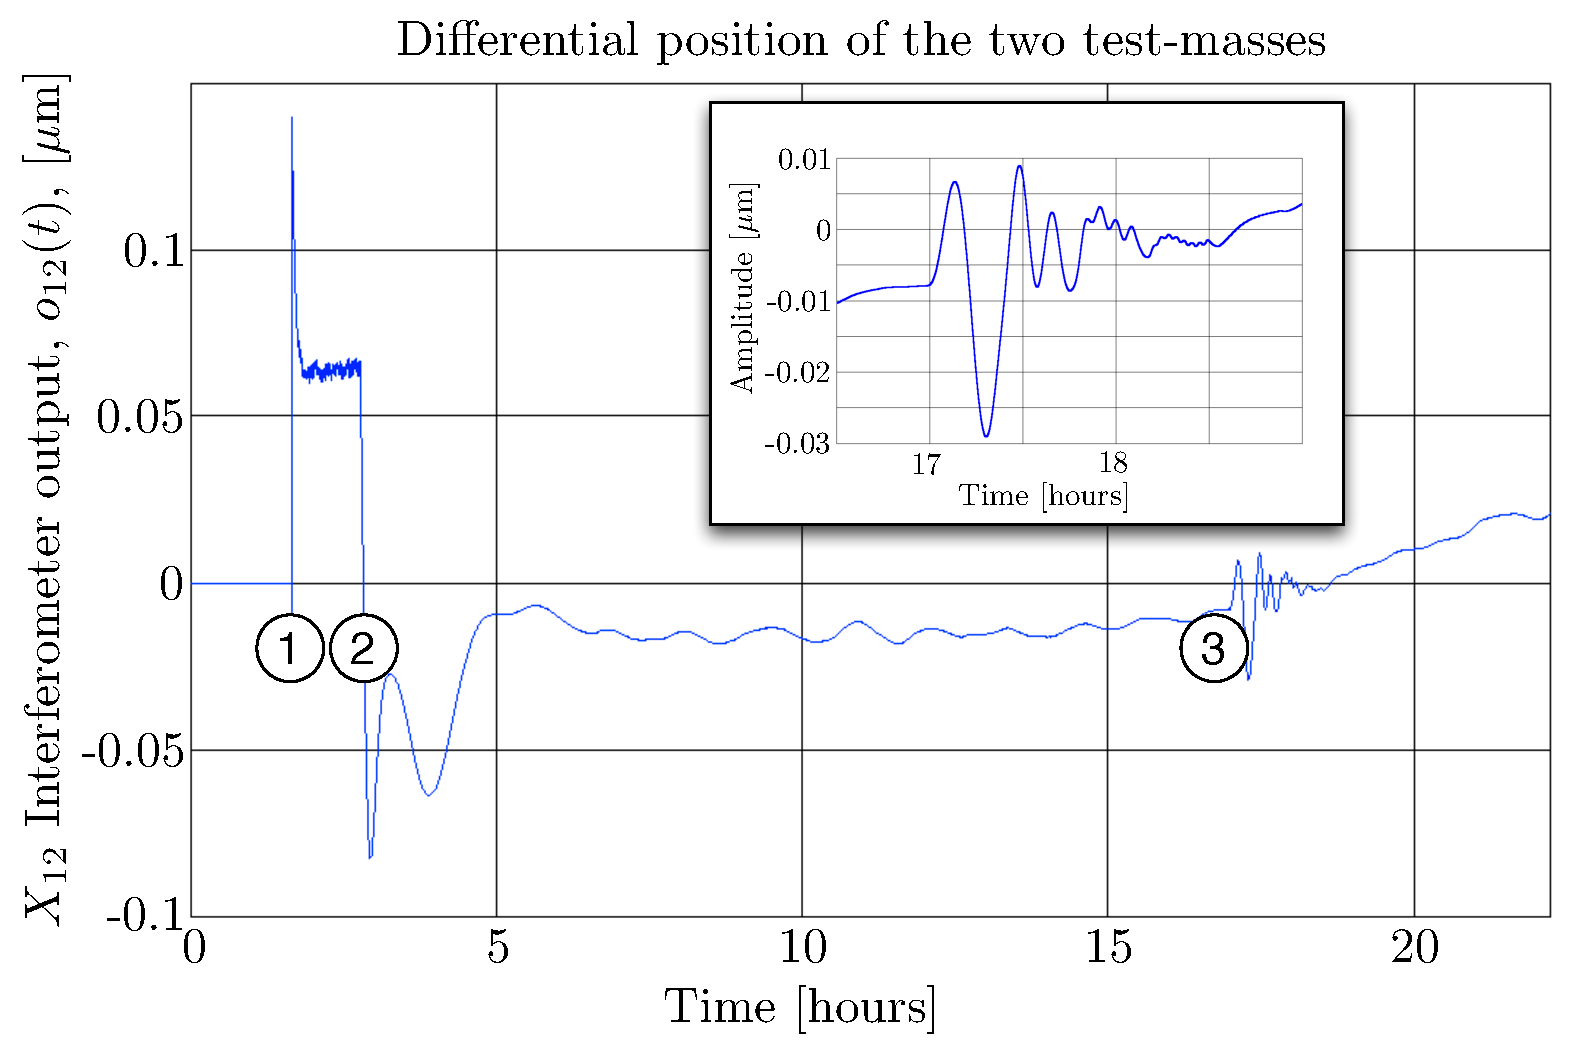
\includegraphics[width=1.0\textwidth]{/Users/hewitson/working/software/cocoa/mac/TeXnicle/TeXnicle/tests/UserManualArticle/o12_1_full.pdf}
\caption{My Nice Figure.}
\label{fig:myfigure}
\end{figure}

some more \nice{text}




